\documentclass[a4paper,12pt]{article}

\usepackage[top=3cm, bottom=2cm, left=3cm, right=2cm]{geometry}
\usepackage[utf8]{inputenc}
\usepackage[portuguese]{babel}
\usepackage{booktabs}
\usepackage{multirow}
\usepackage{hyperref}
\usepackage{graphicx}
\usepackage{longtable}
\usepackage{verbatim}
\usepackage{url}

\usepackage{float}
\floatstyle{ruled}
\newfloat{program}{thp}{lop}
\floatname{program}{Script}

\title{Serviços de Rede e de Sistema \\
Exterior Routing }

\author{André Fernandes (ei03107) \and Miguel Gomes (ei07075) \and Pedro Batista (ext10392)}

\begin{document}

\maketitle

\section{Topologia}

Neste trabalho, a topologia de rede foi ligeiramente alterada face à 
proposta no protocolo. No mesmo é proposto uma configuração do protocolo BGP 
que permitisse interligar todas as 6 bancadas do laboratório. 
Em virtude de termos realizado o trabalho isoladamente decidimos apenas 
interligar 4 bancadas (as primeiras três e a sexta).
No entanto, todos os ASs permaneceram compostos por 4 routers interligados pelo 
protocolo OSPF e distribuidos por duas VLANs, à semelhança do trabalho anterior. 

Na figura \ref{fig:topologia} é possível observar a topologia dos ABR da rede,
bem como o seu endereçamento.

\begin{figure}[htp]
	\begin{center}
		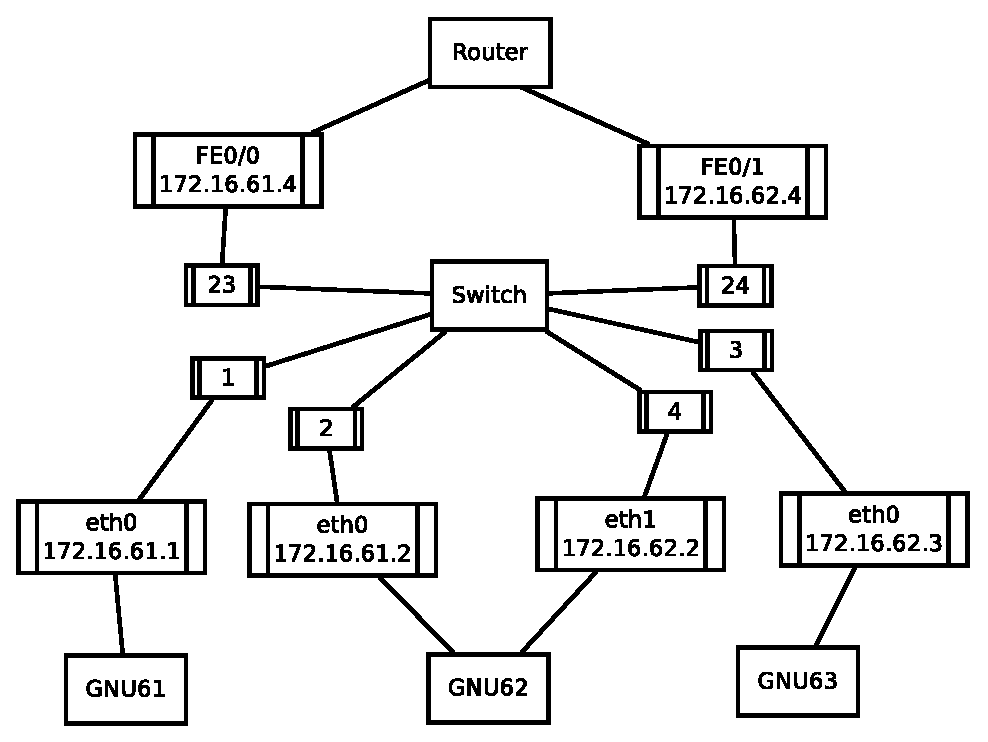
\includegraphics[width=6in]{topologia}
	\end{center}
	\caption{Topologia de rede implementada.}
	\label{fig:topologia}
\end{figure}

\section{Cenários}

Após termos configurado a rede tal como descrito anteriorment, estudámos o comportamento 
da rede em dois cenários diferentes. No primeiro cenário foi analizado o comportamento 
da rede quando cada ABR dá a mesma importância aos seus vizinhos directos.
Já no segundo caso, verificámos como é que o protocolo BGP funciona quando atribuímos
importâncias diferentes aos vizinhos directos. Neste caso, cada ABR deu maior
prioridade aos vizinhos com maior número identificador do AS.

\section{Análise de Tráfego}

No primeiro cenário do trabalho, procedemos de forma incremental. Acrescentando,
progressivamente os routers à rede BGP. Isto permitiu perceber melhor o
funcionamento do protocolo BGP, cujo o funcionamento poderia ser mais díficil 
entender caso não o fizessemos.

Se não tivessemos analizado de forma incremental a adição dos routers no protocolo
BGP poderíamos ter sido induzidos em erro e pensar que estaria a existir algum
problema com a nossa configuração. Uma vez que poderíamos pensar que todos os
ABR teriam de ter dois caminhos para cada outro vizinho do protocolo BGP. 
Ora, isto não é verdade como pode ser verificado pelos logs.

Em qualquer um dos cenários existiram sempre dois routers que continham duas
rotas para cada ABR e outros dois routers em que todas as suas rotas eram únicas.
Isto é, estes routers não tinham rotas alternativas para os outros ABR.

O procedimento efectuado para descobrir isto foi: 
\begin{enumerate}
	\item Ligação do ABR do AS001 com o do AS002.
	\item Ligação do ABR do AS003 com o do AS006.
	\item Ligação do ABR do AS002 e AS006.
	\item E finalmente, a ligação do ABR do AS001 e AS003.
\end{enumerate}

Assim foi possível constatar que as primeiras 3 etapas tiveram a adição das
rotas esperadas em cada um dos ABR. No entanto, os efeito de termos completado
um ciclo na quarta etapa não obteve o resultado que estávamos à espera.
Nomeadamente, a da existência de duas rotas alternativas em cada ABR para cada um
dos outros ABR.

Quando foi adicionada esta última ligação, os ABR das AS003 e AS006, permaneceram
na obscuridade acerca da existência desta ligação. Este comportamento visa,
provavelmente, evitar a existência de ciclos no protocolo.

OU SERÁ QUE TERÁ A VER COM A NÃO EXISTÊNCIA DE PROPAGAÇÂO DAS ROTAS POR TODOS?

\section{Arquivos de log}

Na pasta logs anexada a este arquivo, podemos encontrar os logs e arquivos de
configuração capturados. Para este assumimos a seguinte convenção \verb gX  para
os Gnus (\verb X  representa o respectivo Gnu), \verb r6  para o router cisco, e
\verb s6  para o switch cisco. As pastas \verb logs/cY  representas os três
cenários indicados no guia (\verb Y  varia de 1 a 3 representando os cenários).
Já as pastas \verb logs/cY/trace_route  como o nome indica representa o
trace route de todos os componentes para todos os outros do sistema. Finalmente
as pastas \verb logs/conf/{gX,r6,s6}  mostram as configurações efetuadas no
sistema. Abaixo detalhamos os arquivos de cada pasta.

\begin{itemize}
	\item Para os logs em \verb-logs/cY-
		\begin{description}
			\item \verb *\_zebra  Representa o comando \verb-show ip route-.
			\item \verb *\_ospf  Representa o comando \verb-show ip ospf neighbor-.
		\end{description}
	\item Para os trace routes em \verb-logs/cY/trace_route-
		\begin{description}
			\item \verb {gX,r6}_{gX,r6}[.{61,62}]  Representa o trace route do
				elemento anterior ao \verb _  para o elemento posterior. A parte
				opicional que contém o \verb .  ilustra para o caso do \verb g2  e
				\verb r6  ondo o trace route pode ser feito a rede \verb 61  ou \verb 62 .
		\end{description}
	\item Para as configurações em \verb-logs/confs/gX-
		\begin{description}
			\item[zebra.conf] Apresenta a configuração do zebra no respectivo
				gnu.
			\item[ospfd.conf] Apresenta a configuração ospf no respectivo gnu.
		\end{description}
	\item Para as configurações em \verb-logs/confs/{r6,s6}-
		\begin{description}
			\item[running-config] Apresenta a configuração do router ou switch
				gerada com o comando \verb_show running-config_.
		\end{description}
\end{itemize}

%\bibliographystyle{alpha}
%\bibliography{referencias}

\end{document}
